% !TeX program = lualatex
% Lualatex is important to render Fira fonts; with pdflatex it's just the regular one
\documentclass[12pt]{beamer}

\usetheme{metropolis}
\usepackage{appendixnumberbeamer}

% adjust the background to be completely white
\setbeamercolor{background canvas}{bg=white}

\usepackage{booktabs}
\usepackage[scale=2]{ccicons}

\usepackage{pgfplots}
\usepgfplotslibrary{dateplot}

% typeset mathematics on serif
\usefonttheme[onlymath]{serif}

% better bibliography using biber as backend
\usepackage[natbib=true,backend=biber,style=authoryear-icomp,maxbibnames=30,maxcitenames=3,uniquelist=false,giveninits=true,doi=false,url=true,dashed=false,isbn=false]{biblatex}
% shared bibliogrphy
\addbibresource{../dl4nlp-bibliography.bib}
% disable "ibid" for repeated citations
\boolfalse{citetracker}

% TODOs
\usepackage{todonotes}
\let\todox\todo
\renewcommand\todo[1]{\todox[inline]{#1}}

\definecolor{76abdf}{RGB}{118, 171, 223}

\setbeamercolor{frametitle}{bg=76abdf, fg=white}

\usepackage{xspace}
\newcommand{\themename}{\textbf{\textsc{metropolis}}\xspace}

% POS tags
\newcommand*\POS[1]{\textsubscript{\texttt{#1}}} % tag with part of speech

% parse tree
\usepackage{qtree}

% NNEts
\usepackage{tikz}
\usetikzlibrary{matrix, positioning, calc}

\tikzset{
	neuron/.style={
		draw,
		circle,
		inner sep=0pt,
		minimum width=0.75cm
	},
	layer/.style={
		matrix of nodes,
		nodes={neuron},
		row sep={between origins, 1.2cm}, %1.5cm in general, 2.5cm for backprop task
		nodes in empty cells
	}
}

% for derivatives, https://tex.stackexchange.com/a/412442
\usepackage{physics}

% code listing
\usepackage{listings}

% XML formatting; taken from https://gist.github.com/sebald/3130827
\definecolor{dkgreen}{rgb}{0,0.6,0}
\definecolor{gray}{rgb}{0.5,0.5,0.5}
\definecolor{mauve}{rgb}{0.58,0,0.82}
\definecolor{gray}{rgb}{0.4,0.4,0.4}
\definecolor{darkblue}{rgb}{0.0,0.0,0.6}
\definecolor{lightblue}{rgb}{0.0,0.0,0.9}
\definecolor{cyan}{rgb}{0.0,0.6,0.6}
\definecolor{darkred}{rgb}{0.6,0.0,0.0}
\lstset{
	basicstyle=\ttfamily\scriptsize,
	columns=fullflexible,
	showstringspaces=false,
	numbers=left,                   % where to put the line-numbers
	numberstyle=\tiny\color{gray},  % the style that is used for the line-numbers
	stepnumber=1,
	numbersep=5pt,                  % how far the line-numbers are from the code
	backgroundcolor=\color{white},      % choose the background color. You must add \usepackage{color}
	showspaces=false,               % show spaces adding particular underscores
	showstringspaces=false,         % underline spaces within strings
	showtabs=false,                 % show tabs within strings adding particular underscores
	frame=none,                   % adds a frame around the code
	rulecolor=\color{black},        % if not set, the frame-color may be changed on line-breaks within not-black text (e.g. commens (green here))
	tabsize=2,                      % sets default tabsize to 2 spaces
	captionpos=b,                   % sets the caption-position to bottom
	breaklines=true,                % sets automatic line breaking
	breakatwhitespace=false,        % sets if automatic breaks should only happen at whitespace
	title=\lstname,                   % show the filename of files included with \lstinputlisting;
	% also try caption instead of title  
	commentstyle=\color{gray}\upshape
}
\lstdefinelanguage{XML}
{
	morestring=[s][\color{mauve}]{"}{"},
	morestring=[s][\color{black}]{>}{<},
	morecomment=[s]{<?}{?>},
	morecomment=[s][\color{dkgreen}]{<!--}{-->},
	stringstyle=\color{black},
	identifierstyle=\color{lightblue},
	keywordstyle=\color{red},
	morekeywords={xmlns,xsi,noNamespaceSchemaLocation,type,id,x,y,source,target,version,tool,transRef,roleRef,objective,eventually}% list your attributes here
}


% tables with color
\usepackage{colortbl}


\title{Deep Learning for Natural Language Processing}
\subtitle{Lecture 5 -- Bilingual and Syntax-Based Word Embeddings}
\date{May 11, 2021}
\author{Dr.\ Ivan Habernal}
\institute{Trustworthy Human Language Technologies  \hfill 
\includegraphics[height=.8cm]{img/logo-trusthlt.pdf} \\
Department of Computer Science\\
Technical University of Darmstadt \hfill \texttt{www.trusthlt.org}}
%\titlegraphic{\hfill }

\begin{document}

\maketitle


%\begin{frame}{Table of contents}
%  \setbeamertemplate{section in toc}[sections numbered]
%  \tableofcontents[hideallsubsections]
%\end{frame}

%\section{Administrative course issues}

\begin{frame}{This lecture}
	
Multi-Lingual, Multi-Sense Word Embeddings


Syntactic Word Embeddings


Miscellaneous


\end{frame}


\begin{frame}{Word Senses}
	
\begin{columns}
	
	\begin{column}{6cm}
			Words do not represent only one meaning
			
			\bigskip
			
				Problem is generally known as polysemy (or even homonymy): a word may have many different meanings:

			\begin{itemize}
				\item bank, \textbf{table}, fly, man, ...
			\end{itemize}

	\end{column}

\begin{column}{4cm}

\begin{figure}
	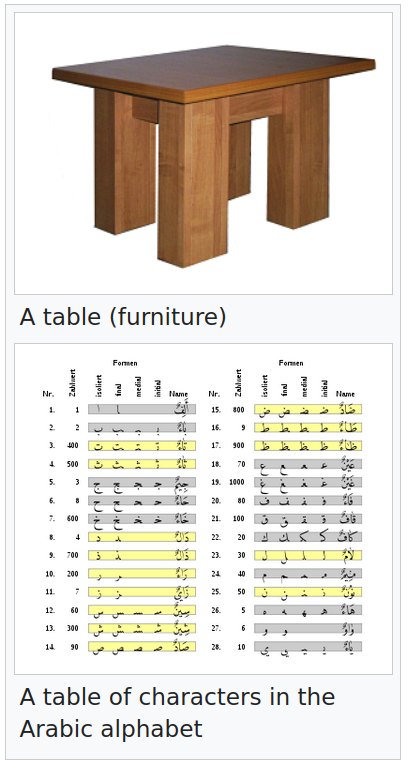
\includegraphics[width=0.8\linewidth]{img/wiktionary-table.png}
	\caption{Source: Wiktionary}
\end{figure}

\end{column}
	
\end{columns}	


	

	
	
	

	
	
\end{frame}


\begin{frame}{Word Senses}

\emph{Man}

\begin{enumerate}
	\item The human species (man vs. other organism)
	\item Males of the human species (i.e. man vs. woman)
	\item Adult males of the human species
\end{enumerate}


This example shows the specific polysemy where the same word is used at different levels of a taxonomy.

Example 1 contains example 2, and example 2 contains example 3.
	
	
\end{frame}

\begin{frame}[fragile]{Sense-disambiguated word representations}
	

Idea: Train word vectors on sense-disambiguated corpora
%Shortened example from the SemCor corpus:

\emph{"a rush of panic caught Sarah"}\footnote{Shortened example from \emph{SemCor} corpus. Not all words have different senses; function words and punctuation do not have senses}


\begin{lstlisting}[language=XML]
<s snum="132">
  <wf pos="DT">A</wf>
  <wf pos="NN" lemma="rush" wnsn="2">rush</wf>
  <wf pos="IN">of</wf>
  <wf pos="NN" lemma="panic" wnsn="1">panic</wf>
  <wf pos="VB" lemma="catch" wnsn="12">caught</wf>
  <wf pos="NNP" lemma="person" wnsn="1">Sarah</wf>
  <punc>.</punc>
</s>
\end{lstlisting}

\vspace*{-3em}
\texttt{=> A rush\_2 of panic\_1 caught\_12 Sarah\_1}


\end{frame}

\begin{frame}{Sense-disambiguated word representations}
	
\begin{figure}
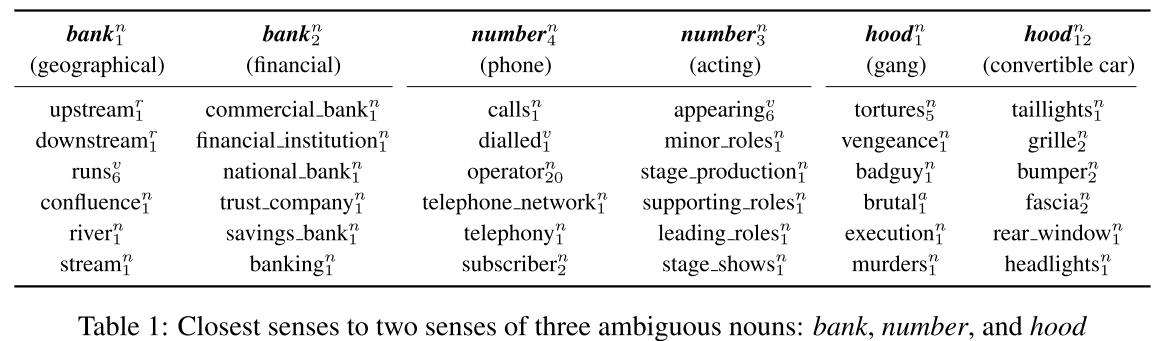
\includegraphics[width=0.95\linewidth]{img/sensembed1.png}
\caption{Result: different representations for each sense\footnote{\fullcite{Iacobacci.et.al.2015.ACL}}}
\end{figure}

Note: subscript is sense-id superscript is pos-tag
Number and bank could also appear as verbs (not illustrated here)

	
\end{frame}


\begin{frame}{Problems}
How do you now train an NLP system with these sense-disambiguated embeddings?

\end{frame}


\begin{frame}{A more parsimonious approach}

	Run word2vec on your data and compute embeddings
	
	For each target word, represent its context as avg. or concatenated embedding
	
\begin{itemize}
	\item ... need to go to the \emph{bank} to get some money ...
	\item ... debt by utilizing a credit line granted by a \emph{bank} ...
	\item ... raw water is largely river \emph{bank} filtrate (approximately 70 percent) ...
	\item ... runs from its idyllic river \emph{bank} promenade under the Elbe to ...
\end{itemize}

	
\end{frame}

\begin{frame}{A more parsimonious approach}
	
	Run word2vec on your data and compute embeddings
	
	For each target word, represent its \textbf{context} as avg. or concatenated embedding
	
	\begin{itemize}
	\item ... need \textbf{to go to the} \emph{bank} \textbf{to get some money} ...
\item ... debt by utilizing a \textbf{credit line granted by a} \emph{bank} ...
\item ... raw \textbf{water is largely river} \emph{bank} \textbf{filtrate (approximately 70 percent}) ...
\item ... runs \textbf{from its idyllic river} \emph{bank} \textbf{promenade under the Elbe} to ...
	\end{itemize}
	
\end{frame}

\begin{frame}{A more parsimonious approach}
	
	\begin{itemize}
		\item ... need \textbf{to go to the} \emph{bank} \textbf{to get some money} ... $\to [.2,.8]$
		\item ... debt by utilizing a \textbf{credit line granted by a} \emph{bank} ... $\to [.4,.6]$
		\item ... raw \textbf{water is largely river} \emph{bank} \textbf{filtrate (approximately 70 percent}) ... $\to [-.2,-.8]$
		\item ... runs \textbf{from its idyllic river} \emph{bank} \textbf{promenade under the Elbe} to ... $\to [-.9,-.3]$
	\end{itemize}

Cluster the context representations (unsupervised!)

Assign each word’s context to a cluster: the word has the sense corresponding to the cluster index

Run word2vec on sense-disambiguated corpus 
	
\end{frame}

\begin{frame}{Sense-disambiguated word representations}

Promising approach to unsupervised sense-disambiguated word representation

On the other hand, the cost is much higher --- one needs a sense-labeler or a more complicated model

Hardly used in practice

Before ELMo and BERT came around in 2018 with \textbf{contextualized word embeddings}

\end{frame}


\begin{frame}{Bilingual Embeddings}
	
Word representations for two languages: 

train on corpus from both languages

\begin{figure}
	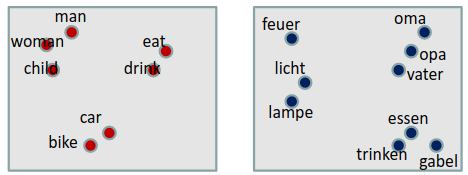
\includegraphics[width=0.6\linewidth]{img/biling-1.png}
\end{figure}
	
	
\end{frame}

\begin{frame}{Bilingual Embeddings}
	
Goal: represent words from different languages in the same space

	
	\begin{figure}
		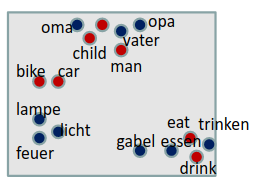
\includegraphics[width=0.4\linewidth]{img/biling-2.png}
	\end{figure}
	
	
\end{frame}

\begin{frame}{Bilingual Embeddings -- General idea}
	
Can think of it as having two objectives we want to satisfy
	
\begin{itemize}
	\item \textbf{cross-lingual objective}: words that are translations of each other should be close in the projected space
	\item \textbf{mono-lingual objective}: words that occur in monolingually similar contexts should be close to each other in vector space
\end{itemize}	
	
	
\end{frame}


\begin{frame}{Bilinguality -- Why?}
	
(1) Second language may act as an additional "signal"

\begin{itemize}
	\item Which may help to improve word embeddings even in the first language \\
	$\to$ \emph{Make Monolingual Embeddings better}
	\item E.g. assume that some word like “opa” occurs very infrequently in the German corpus, thus it’s difficult to reliably estimate its word embedding
	\item If its English translation “grandfather” occurs frequently in the English corpus, the German word should get a more appropriate embedding in the bilingual space
\end{itemize}

\end{frame}


\begin{frame}{Bilinguality -- Why?}
	
(2) If words are projected in a common space (“shared features”), this may allow for \textbf{direct transfer} 

\begin{itemize}
	\item Train a model in one language (usually resource-rich)
	\item Directly apply in another language (usually resource-poor)
\end{itemize}

\end{frame}


\begin{frame}{Bilinguality -- Example}
(2) Example Direct Transfer: task is POS tagging
	
Goal / approach: 

Train: \emph{I may not drink this} $\to$ PRON VERB PARTICLE VERB DET

Test: \emph{Es ist wichtig, ausreichend zu trinken} $\to$ ?



\begin{block}{Training (idea):}
	
	\begin{columns}
		\column{6cm}
		
		Input: center words with their context words

		Output: labels of center word
		
		E.g. (not, \textbf{drink}, this) $\to$ VERB
		
		\column{3cm}
		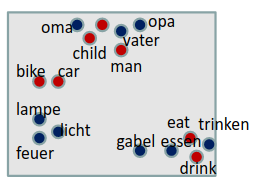
\includegraphics[width=\linewidth]{img/biling-2.png}
		
	\end{columns}
\end{block}

\end{frame}

\begin{frame}{Bilinguality -- Example}
(2) Example Direct Transfer: task is POS tagging

Direct transfer aka zero-shot transfer: 

- train using bilingual embeddings in English (assume big labeled English dataset) 

- then apply to German data

Problems with the Direct Transfer approach?

- "OOV words"

- syntactic ordering

	
\end{frame}


\begin{frame}{Bilingual Embeddings – Naive Approach}
	
Given 1: Monolingual Embeddings (e.g. English, German)

Given 2: Dictionary EN $\Leftrightarrow$ DE
	
Translate German words to English words, assign them the embedding of the English word (or concatenate, average, ...)


\begin{itemize}
	\item 	Bottleneck is the dictionary
	\item 	Cannot assign meanings to words that are not in the dictionary
\end{itemize}
	
	
\end{frame}


\begin{frame}{Bilingual Embeddings}
	
	More sophisticated approaches have been suggested, relying on different kinds of (costly) information
	
\end{frame}


\begin{frame}{Approach 1: Learning a transformation matrix}

\begin{itemize}
	\item One of the first and simplest approaches
	\begin{itemize}
		\item Mikolov et al. 2013, Exploiting similarities among languages for machine translation
	\end{itemize}
\end{itemize}

\begin{itemize}
	\item Given: monolingual embeddings + dictionary 
	\begin{itemize}
		\item Dictionary: cat-Katze, table-Tisch, …
	\end{itemize}
\end{itemize}

\begin{table}
\begin{tabular}{l|l}
$x_i$ & $z_i$ \\ \hline
cat & Katze \\ \hline
table & Tisch \\ \hline
... & ... \\
\end{tabular}
\end{table}

\end{frame}


\begin{frame}{Approach 1: Learning a transformation matrix}
	
	\begin{table}
		\begin{tabular}{l|l}
			$\mathbf{x}_i$ & $\mathbf{z}_i$ \\ \hline
			$[0.2,-0.3,0.8]$ & $[0.5,0.9,-1]$ \\ \hline
			$[1,2,-5]$ & $[0.1,-0.1,0.1]$ \\ \hline
			... & ... \\
		\end{tabular}
	\end{table}
	
We estimate a linear transformation from this data:

$$
\min_{\mathbf{W}} \sum_i \norm{\mathbf{x}_i \mathbf{W} - \mathbf{z}_i}_2
$$

- $\mathbf{x}_i$ and $\mathbf{z}_i$: monolingual word vectors from dictionary

Once $ \mathbf{W}$ is learned, we can map any language $\mathbf{x}$ word into the space of
language $\mathbf{z}$

Even words for which we do not have translations
	
\end{frame}

\begin{frame}{More Bilingual Embeddings -- Survey papers}

See \fullcite{Upadhyay.et.al.2016.ACL}

And more recent \fullcite{Glavas.et.al.2019.ACL}


\end{frame}

\begin{frame}{Bilingual embeddings}
	
\textbf{BiSkip} uses sentence and word aligned texts, then runs a skip-gram model
whose contexts are words from both languages:

\begin{itemize}
	\item E.g. on input \emph{love} BiSkip wants to predict the context \emph{je}, \emph{I}, \emph{you}, \emph{t’};
	\item similar for \emph{aime}: \emph{t’}, \emph{you}
	\item $\to$ similar contexts are predicted $\to$ similar representations
\end{itemize}
	
\begin{figure}
	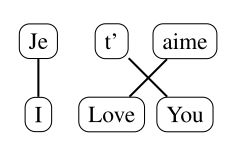
\includegraphics[width=0.3\linewidth]{img/biskip.png}
\end{figure}
\end{frame}


\begin{frame}{Bilingual embeddings}
	
	\textbf{BiVCD}\footnote{\fullcite{Vulic.Moens.2015.ACL}} is even simpler. Given aligned documents (e.g. Wikipedia articles)
	
	\begin{itemize}
		\item Merge them, then random shuffle all words
		\item Then run a Monolingual Model (e.g. CBOW, Glove, Skip-Gram) on it
	\end{itemize}
	
	
	\begin{figure}
		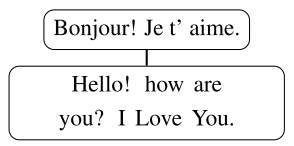
\includegraphics[width=0.3\linewidth]{img/bivcd.png}
	\end{figure}
\end{frame}


\begin{frame}{Determining bi-lingual mappings (for BiSkip)}
	
Dictionary

Inter-lingual links in Wikipedia

Word alignments learned from parallel corpora
	
\end{frame}


\begin{frame}{Multilinguality}

\begin{itemize}
	\item  We talked about mapping two languages in a common space
	\item How about 3, 5, 10 languages?
	\item Much less explored topic
	\item However, there is work on it, such as Ammar et al. (2016), Massively Multilingual word embeddings
	\begin{itemize}
		\item They extend BiCCA to MultiCCA and BiSkip to MultiSkip 
	\end{itemize}
\end{itemize}

In recent years, Multilingual BERT (MBERT), which yields embeddings in a joint space for 100+ languages

\end{frame}


\begin{frame}{Current trends}
	
\begin{itemize}
	\item Learn bilingual word embeddings from as few resources as possible
	\item E.g., only 10 aligned word pairs (can be punctuation)
	\item From there we can go to unsupervised machine translation
\end{itemize}
	
\end{frame}

\begin{frame}{Current trends}
	
\fullcite{Artetxe.et.al.2017.ACL}

Main idea:

-- If we had a dictionary, we can get bilingual embeddings

-- If we had bilingual embeddings, we can get a dictionary 


\end{frame}

\begin{frame}{Current trends}
	
\citeauthor{Artetxe.et.al.2017.ACL}'s (\citeyear{Artetxe.et.al.2017.ACL}) method:
	
\begin{enumerate}
	\item Use a lexicon (seed lexicon is easy to get automatically)
	\item Learn bilingual embeddings using current lexicon ($\to$ Mikolov’s method, i.e., “Approach 1”)
	\item Get a better lexicon using bilingual embeddings
	\item Go back to 1)
\end{enumerate}

\begin{figure}
	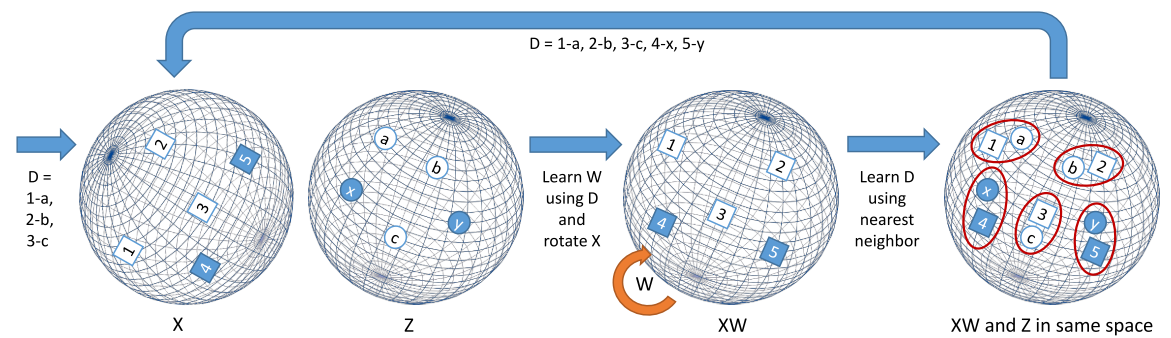
\includegraphics[width=0.8\linewidth]{img/artetxe.png}
\end{figure}
	
	
\end{frame}

\section{Syntactic word embeddings}

\begin{frame}{More syntactically oriented embeddings}
Syntactic relations between words should also be represented in the vectors

-- Problem: word order matters

\emph{Dog bites man.} \hspace{2em} vs. \hspace{2em} \emph{Man bites dog.}
	

\end{frame}

\begin{frame}{Position Information}

Remember: The \texttt{word2vec} models do not consider position information: 

\begin{itemize}
	\item No distinction between left and right context
	\item No distinction between close and far contexts
\end{itemize}



Skip-gram: \underline{~~~~~~} bites \underline{~~~~~~} \\
$\to$ (bites, man) , (bites, dog)


\end{frame}



\begin{frame}{Position Information}
	
	
\emph{dog bites man} \hspace{2em} vs. \hspace{2em} \emph{man bites dog}
	

\texttt{(bites, dog-1), (bites, man+1)}

vs.


\texttt{(bites, man-1), (bites, dog+1)}
	

This is “intuitively” what we want (although we don't add indices to words)
	
\end{frame}


\begin{frame}{Skip-gram model}
	
\begin{columns}
	
	\begin{column}{4cm}
		\begin{figure}
			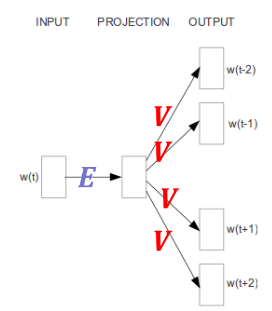
\includegraphics[width=\linewidth]{img/skipgram1.png}
			\caption{SkipGram model}
		\end{figure}
	\end{column}
	
	\begin{column}{4cm}
How can we predict different words when V is always the same?
	\end{column}
	
\end{columns}
	
\end{frame}

\begin{frame}{Structured Skip-gram model}
	
	\begin{columns}
		
		\begin{column}{4cm}
			\begin{figure}
				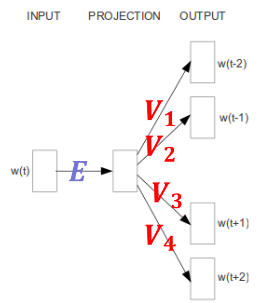
\includegraphics[width=\linewidth]{img/skipgram2.png}
				\caption{Structured SkipGram model}
			\end{figure}
		\end{column}
		
		\begin{column}{4cm}

		\end{column}
		
	\end{columns}
	
\end{frame}


\begin{frame}{Results}
	

Nearest neighbours for \emph{breaking}


\begin{table}
	\begin{tabular}{l|l}
		\rowcolor{76abdf} \textcolor{white}{\textbf{Skip-gram}} & \textcolor{white}{\textbf{Structured Skip-gram}} \\ \toprule
		breaks & putting \\
		\rowcolor{gray!10} turning & turning \\
		broke & sticking \\
		\rowcolor{gray!10} break & pulling \\
		stumbled & picking \\
		\bottomrule
	\end{tabular}
\end{table}

\begin{small}
	Word representations with positional information work slightly better for syntactic tasks like POS-tagging and parsing.
\end{small}

\fullcite{Ling.et.al.2015.NAACL}

	
\end{frame}

\begin{frame}{Long-distance dependencies}
Words can be similar with respect to verb selection preferences

-- tea/milk/beer/coffee can all be an object of the verb \emph{drink}

Words that share syntactic relations might be distant in a sentence:

\emph{I would like to \textbf{drink} a very hot tall decaf half-soy (...insert any other thousand options ...) white chocolate \textbf{mocha}}

\end{frame}

\begin{frame}{Dependency parsing in one slide}
Grammatical relationships between words in a sentence

\begin{figure}
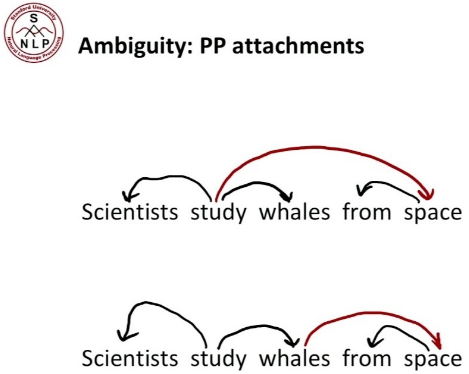
\includegraphics[width=0.5\linewidth]{img/deptree1.png}
\caption{Prepositional phrase (PP) attachment. Image courtesy of Stanford NLP lab}
\end{figure}


\end{frame}


\begin{frame}[fragile]{Towards dependency-embeddings}

Idea: apply dependency parsing first 

\emph{I would like to \textbf{drink} a very hot tall decaf half-soy (...) white chocolate \textbf{mocha}}

Output of Stanford dependency parser:

\begin{tiny}
\begin{verbatim}
nsubj(like-3, I-1)	 	nsubj(drink-5, I-1)	 	aux(like-3, would-2)	 
root(ROOT-0, like-3)	mark(drink-5, to-4)	 	xcomp(like-3, drink-5)	 
det(mocha-14, a-6)	 	advmod(hot-8, very-7)	amod(mocha-14, hot-8) 
amod(mocha-14, tall-9)	amod(mocha-14, decaf-10)	amod(mocha-14, half-soy-11)	
amod(mocha-14, white-12)	compound(mocha-14, chocolate-13)	 
dobj(drink-5, mocha-14)
\end{verbatim}
\end{tiny}
	
\texttt{dobj(drink-5, mocha-14)}: direct object

\begin{small}
The direct object of a verb phrase is the noun phrase which is the (accusative) object of the verb.	
\end{small}


\end{frame}


\begin{frame}[fragile]{Dependency-based embeddings}
	

	\emph{I would like to \textbf{drink} a very hot tall decaf half-soy (...) white chocolate \textbf{mocha}}

	\begin{tiny}
		\begin{verbatim}
		nsubj(like-3, I-1)	 	nsubj(drink-5, I-1)	 	aux(like-3, would-2)	 
		root(ROOT-0, like-3)	mark(drink-5, to-4)	 	xcomp(like-3, drink-5)	 
		...
		\end{verbatim}
	\end{tiny}
	
\begin{small}
	
\fullcite{Levy.Goldberg.2014.ACL}

\begin{table}
	\begin{tabular}{l|l}
		\rowcolor{76abdf} \textcolor{white}{\textbf{Word}} & \textcolor{white}{\textbf{Dependency Context}} \\ \toprule
		like & I/nsubj, would/aux, drink/xcomp \\
		\rowcolor{gray!10} drink & I/nsubj, to/mark,  mocha/dobj, like/xcomp-1 \\
		hot & very/advmod, mocha/amod-1 \\
		\rowcolor{gray!10} ... & ... \\
	\end{tabular}
\end{table}
\end{small}
	
\end{frame}

\begin{frame}{Dependency-based embeddings}

\begin{columns}
	
\begin{column}{4cm}
\texttt{Word2Vec} finds words that \textbf{associate with} other words, while DepEmbeddings finds words \textbf{behave like} others

-- Domain similarity vs. functional similarity
\end{column}

\begin{column}{6cm}
\begin{figure}
	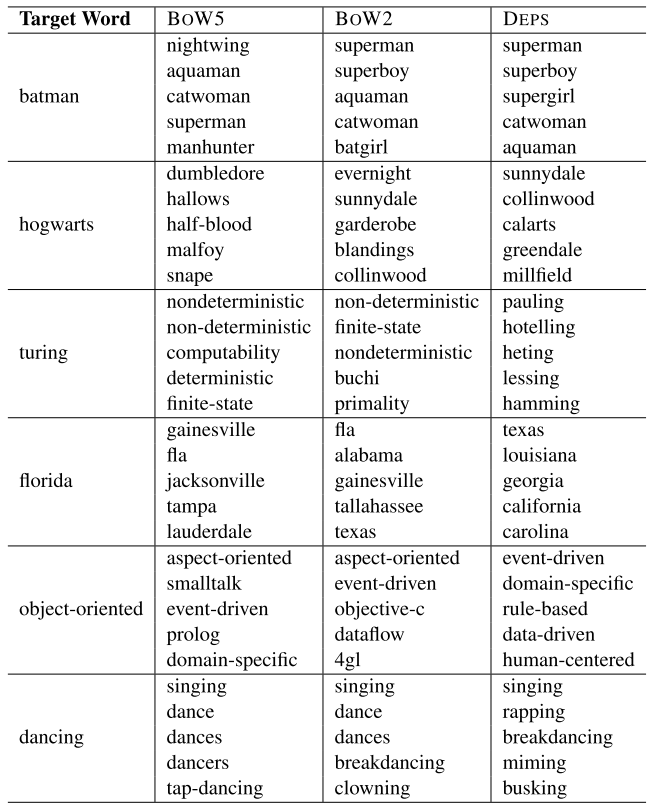
\includegraphics[width=\linewidth]{img/levy2015.png}
\end{figure}
	
\end{column}

\end{columns}
	
\end{frame}

\section{Miscellaneous}


\begin{frame}{Embeddings of other things than words}

Embed other stuff than words:

\begin{itemize}
\item \textbf{Characters}: \emph{i n s i g h t f u l}
\item \textbf{Syllables}: \emph{in + sight + ful} 
\item \textbf{Morphemes}:
\begin{itemize}
	\item \emph{insightful = insight + ful}
	\item \emph{helping = help + ing}
	\item \emph{greedily = greedy + ly}
	\item \emph{Dampfschifffahrt = Dampf+Schiff+Fahrt}
	\item Useful particulary for morphologically rich languages like German, French, Czech, etc.
	\item Rarely find Dampfschifffahrt in a corpus, but its three morphemes are quite likely
\end{itemize}
\item Embed \textbf{postags}, \textbf{synsets}, \textbf{lexemes}, \textbf{supersenses}, ...
\end{itemize}	
\end{frame}


\begin{frame}{Embeddings of other things than words}
	
	
	Embed \textbf{n-grams} -- the \texttt{FastText} approach\footnote{
	\fullcite{Bojanowski.et.al.2017.TACL}}
	
	Words are represented as bags of character n-grams (n=3,4,5,6)
	
	
\begin{small}
n=3: \emph{where} = (  \emph{>wh , whe, her, ere , re<}  )
\end{small}

Learn embeddings for all n-grams, represent a word by averaging over its n-gram embeddings
	

\begin{small}
	Big advantage:
	
	-- 	Can embed OOV words, spelling mistakes: “lenght”, “spellling”  \\
	-- 	Naturally works for morphologically rich languages
\end{small}	
	
\end{frame}




\section{Using word embeddings in a task}


\begin{frame}{Training word vectors to the task}


Option 1: fixed word representations

\begin{itemize}
	\item map word into id and get the vector from the embedding matrix
	\item only train the weights of the hidden layers
\end{itemize}


Option 2:  adjust the word representations to the task

\begin{itemize}
	\item word vectors are parameters and are updated in each epoch
	\item Example: sentiment classification, train vectors to represent positive/negative polarity for each word 
\end{itemize}

\end{frame}



\begin{frame}{Problem: Adaptation to the training data}
	
Representations for words that are seen in the training data move in vector space, but words that are not seen remain where they were

\begin{columns}
	
	\begin{column}{6cm}
		\begin{small}

		\begin{itemize}
			\item “TV”, “telly” and “television” all indicate negative 	sentiment in the dataset
			\item Due to pre-training, they have similar vectors
			\item “TV” and “telly” occur in the training data,	“television” in the test data
		\end{itemize}
		\end{small}
		
	\end{column}
	\begin{column}{5cm}
		\begin{figure}
			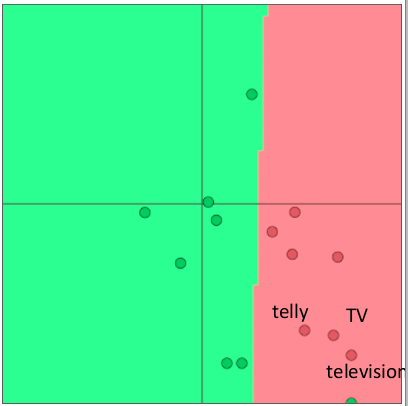
\includegraphics[width=0.8\linewidth]{img/socher1.png}
			\caption{Courtesy of Richard Socher}
		\end{figure}	
		
	\end{column}
	
\end{columns}

\end{frame}


\begin{frame}{Problem: Adaptation to the training data}
	
	“TV” and “telly” have been updated
	
	“television” stayed the same -> synonym information is lost
	
	
	\begin{columns}
		
		\begin{column}{5cm}
			\begin{figure}
				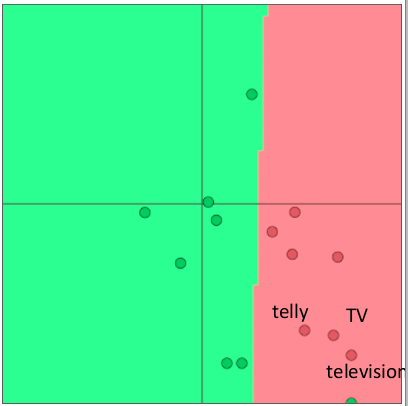
\includegraphics[width=0.8\linewidth]{img/socher1.png}
				\caption{Before training}
			\end{figure}	
			
			
		\end{column}
		\begin{column}{5cm}
			\begin{figure}
				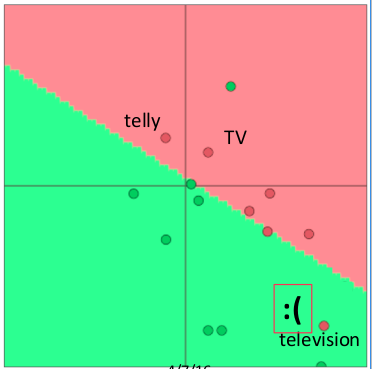
\includegraphics[width=0.8\linewidth]{img/socher2.png}
				\caption{After training}
			\end{figure}	
			
		\end{column}
		
	\end{columns}
	
\end{frame}


\begin{frame}{Practical tips}
	
Only train word vectors to the task if you have a large training corpus.

Even then, it might not be useful (depends on the task).

\bigskip

Common practice: 

-- Train the vectors only for a few epochs and then keep them fixed

\begin{block}{If in doubt}
	Keep your embeddings fixed
\end{block}


\end{frame}

\section{Summary}

\begin{frame}{Summary: Embedding approaches}
What do all the embedding approaches have in common? 

-- Represent natural language input with real-valued vectors

Differences

\begin{exampleblock}{Unit of representation}
characters, morphemes, words, senses, phrases, windows, sentences, documents, ...
\end{exampleblock}

\begin{exampleblock}{Definition of context for training}
CBOW, Skip-gram, Glove, positional, dependency-based, ...
\end{exampleblock}


\end{frame}

	
\begin{frame}{Towards contextualized embeddings}

Static word embeddings -- huge impact on adoption of DL in NLP

Becoming extinct now

Deplaced by contextualized embeddings (BERT, etc.)
	
\end{frame}

\begin{frame}{License and credits}

\begin{columns}
	\begin{column}{0.7\textwidth}
		Licensed under Creative Commons Attribution-ShareAlike 4.0 International (CC BY-SA 4.0)
	\end{column}
	\begin{column}{0.2\textwidth}
		
\includegraphics[width=0.9\linewidth]{img/cc-by-sa-icon.pdf}
	\end{column}
\end{columns}

\bigskip

Credits

\begin{scriptsize}
	
Ivan Habernal, Steffen Eger

Akir (\url{https://commons.wikimedia.org/wiki/File:Table.png}, CC-BY-SA)

Baba66 (\url{https://commons.wikimedia.org/wiki/File:Arabicalphabet.svg}, CC-BY)

Content from ACL Anthology papers licensed under CC-BY \url{https://www.aclweb.org/anthology}

\end{scriptsize}

\end{frame}

\begin{frame}[allowframebreaks]{References}
\printbibliography
%  \bibliography{bibliography}
%  \bibliographystyle{abbrv}
\end{frame}

\end{document}

